\documentclass[12pt, a4paper]{article}
\usepackage[utf8]{inputenc}
\usepackage[T1]{fontenc}
\usepackage[brazil]{babel}
\usepackage{lmodern}
\usepackage{microtype}
\usepackage{geometry}
\geometry{margin=2.5cm}
\usepackage{amsmath, amssymb}
\usepackage{booktabs}
\usepackage{array}
\usepackage{multirow}
\usepackage{hyperref}
\hypersetup{colorlinks=true, linkcolor=blue!60!black, urlcolor=blue!60!black}
\usepackage{xcolor}
\usepackage{parskip}
\setlength{\parskip}{6pt}
\usepackage{enumitem}
\setlist{nosep, leftmargin=1.5em}
\usepackage{titlesec}
\titleformat{\section}{\large\bfseries}{}{0em}{}[\titlerule]
\titleformat{\subsection}{\normalsize\bfseries}{}{0em}{}
\usepackage{graphicx}
\graphicspath{{figs/}}
\usepackage{caption}
\captionsetup{font=small, labelfont=bf, skip=4pt}
\usepackage{float}

% ── Comandos utilitários ──────────────────────────────────────────────
\newcommand{\alg}[1]{\textsc{#1}}
\newcommand{\nfe}{\mathrm{NFE}}
\newcommand{\fref}{f^{*}}
\newcommand{\lam}{\lambda}
\newcommand{\err}{e}

\title{\textbf{Metaheurísticas Recentes em Problemas de Engenharia com Restrições}\\[4pt]
       \large Interpretação dos Resultados Experimentais}
\author{Otimização Estocástica --- Doutorado}
\date{\today}

\begin{document}
\maketitle
\tableofcontents
\newpage

% ═══════════════════════════════════════════════════════════════════════
\section{Contexto e objetivos}

Este documento interpreta os resultados dos quatro experimentos do
notebook \texttt{metaheuristicas\_engenharia\_nfe.ipynb}, que compara
cinco metaheurísticas publicadas em~2025 em problemas de engenharia
com restrições. Os experimentos foram executados em Python~3.14.7
com NumPy~2.5.4, SciPy~1.18.1 e Pandas~3.0.6, em máquina com 12~núcleos.
Os cinco algoritmos avaliados são:

\begin{itemize}
  \item \alg{BfOA} — Battlefield Optimization Algorithm
  \item \alg{CCO} — Cuckoo Catfish Optimizer
  \item \alg{LMO} — Logarithmic Mean Optimization
  \item \alg{ODO} — Offensive--Defensive Optimization
  \item \alg{TIEO} — Tribal Intelligent Evolution Optimization
\end{itemize}

Os experimentos progridem do \emph{protocolo original do artigo} (Exp.~A)
para comparações cada vez mais rigorosas: orçamento de avaliações
equalizado~(B), conjunto ampliado de problemas com duas estratégias de
tratamento de restrições e testes estatísticos robustos~(C), e
escalabilidade em funções de maior dimensão~(D).

O erro relativo de cada execução é definido como
\[
  \err = \frac{F - \fref}{|\fref|},
\]
com $F$ o valor da função efetivamente otimizada (penalizada ou de
Deb) e $\fref$ o ótimo recalculado por SLSQP com 100 partidas
aleatórias. Os valores de referência obtidos são consistentes com a
literatura; a maior diferença ocorre no \textbf{I-Beam (formulação
correta)}, onde $\fref = 0{,}013074$, enquanto o artigo usa uma
formulação com erro tipográfico que resulta em $\fref = 0{,}01493$.
Quando $\fref = 0$, usa-se o erro absoluto.

% ═══════════════════════════════════════════════════════════════════════
\section{Experimento A — Reprodução do Protocolo Original}

\subsection{Critério de parada e consumo de $\nfe$}

O artigo original encerra cada execução após $T = 500$ iterações,
sem fixar o número de avaliações de função ($\nfe$). A tabela~\ref{tab:nfe_a}
mostra o $\nfe$ médio obtido por cada algoritmo em cada problema,
com o valor reportado no artigo entre parênteses.

\begin{table}[h!]
\centering
\caption{Exp.~A — $\nfe$ médio (valor do artigo).}
\label{tab:nfe_a}
\small
\begin{tabular}{lrrrrr}
\toprule
Problema & \alg{BfOA} & \alg{CCO} & \alg{LMO} & \alg{ODO} & \alg{TIEO} \\
\midrule
Welded Beam     & 16\,500 (21\,616) & 15\,030 (15\,297) & 15\,030 & 15\,030 & 11\,614 (10\,855) \\
Cantilever Beam & 16\,500 (21\,616) & 15\,030 (15\,273) & 15\,030 & 15\,030 & 8\,302 (8\,958) \\
Three-Bar Truss & 16\,500 (21\,616) & 15\,030 (15\,271) & 15\,030 & 15\,030 & 8\,334 (9\,350) \\
I-Beam (artigo) & 16\,500 (21\,616) & 15\,030 (15\,300) & 15\,030 & 15\,030 & 12\,120 (11\,741) \\
Tubular Column  & 16\,500 (21\,616) & 15\,030 (15\,309) & 15\,030 & 15\,030 & 11\,409 (9\,673) \\
\bottomrule
\end{tabular}
\end{table}

O \alg{BfOA} consome consistentemente ${\approx}10\%$ mais avaliações
que \alg{CCO}, \alg{LMO} e \alg{ODO} (razão $\approx 1{,}1$) e cerca
de $20$--$40\%$ mais que o \alg{TIEO} (razão $\approx 1{,}4$--$2{,}0$).
Isso ocorre porque o \alg{BfOA} realiza uma fase de reconhecimento
aéreo inicial ($2\,000$~avaliações) somada a $29$~avaliações por
iteração (21 na defesa e~8 no ataque). A comparação baseada em
iterações estruturalmente favorece o \alg{BfOA}, que dispõe de um
orçamento significativamente maior.

\begin{figure}[H]
  \centering
  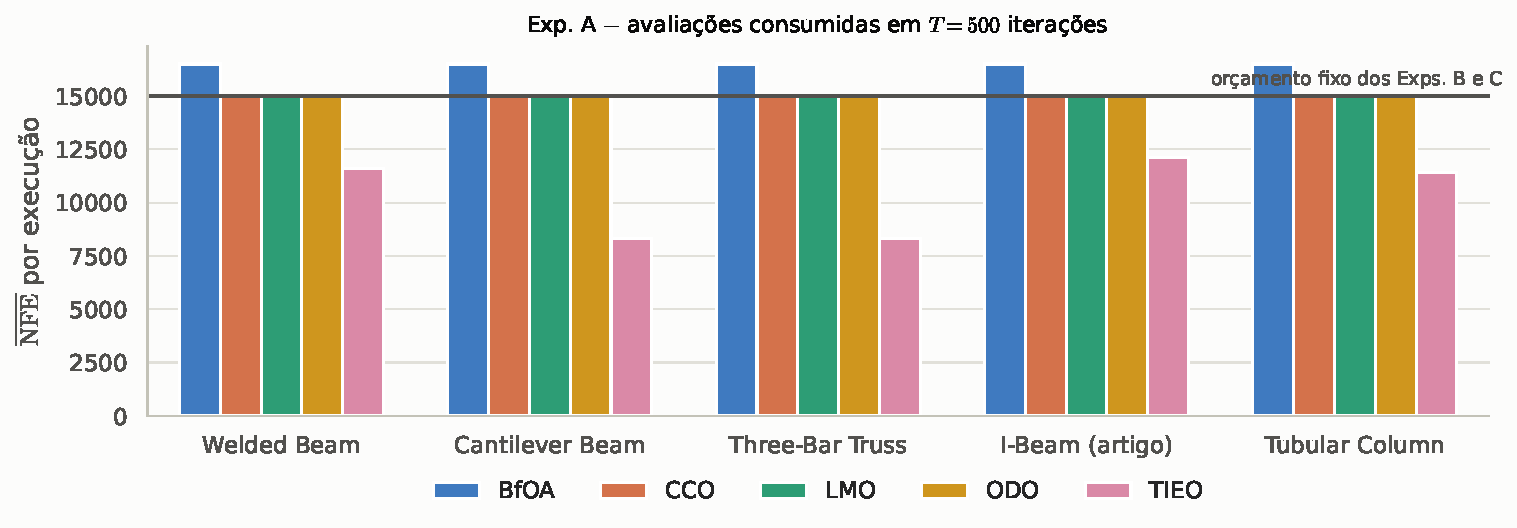
\includegraphics[width=\textwidth]{fig_exp_a_nfe}
  \caption{Exp.~A — $\overline{\nfe}$ médio por algoritmo e problema em $T=500$ iterações.
           A linha tracejada indica o orçamento fixo $\nfe_{\max}=15\,000$ adotado nos Exps.~B e~C.}
  \label{fig:exp_a_nfe}
\end{figure}

\subsection{Qualidade das soluções}

A tabela~\ref{tab:exp_a} resume os resultados por problema no Exp.~A.
Todos os algoritmos retornaram $100\%$ de soluções viáveis
($\max_i g_i(\mathbf{x}) \le 10^{-8}$) em todas as execuções.

\begin{table}[h!]
\centering
\caption{Exp.~A — média e desvio padrão do valor da função objetivo
  (30 execuções). A referência SLSQP é indicada abaixo do nome do problema.}
\label{tab:exp_a}
\small
\begin{tabular}{llrrrrr}
\toprule
Problema & Estat. & \alg{BfOA} & \alg{CCO} & \alg{LMO} & \alg{ODO} & \alg{TIEO} \\
\midrule
Welded Beam & Média & 1{,}7478 & \textbf{1{,}7249} & 1{,}7466 & 1{,}8133 & 1{,}9189 \\
($\fref=1{,}72485$) & DP & 4{,}64e-02 & 8{,}27e-05 & 1{,}46e-02 & 1{,}27e-01 & 2{,}29e-01 \\
\midrule
Cantilever Beam & Média & 1{,}34029 & \textbf{1{,}33996} & 1{,}34253 & 1{,}33999 & 1{,}34010 \\
($\fref=1{,}33996$) & DP & 1{,}61e-04 & 6{,}76e-06 & 1{,}67e-03 & 1{,}79e-05 & 1{,}08e-04 \\
\midrule
Three-Bar Truss & Média & 263{,}897 & \textbf{263{,}8958} & 263{,}902 & 263{,}8963 & 263{,}8973 \\
($\fref=263{,}896$) & DP & 2{,}18e-03 & 9{,}96e-07 & 4{,}62e-03 & 5{,}67e-04 & 1{,}85e-03 \\
\midrule
I-Beam (artigo) & Média & 0{,}014929 & \textbf{0{,}014927} & 0{,}014935 & 0{,}014927 & 0{,}015435 \\
($\fref=0{,}014927$) & DP & 7{,}83e-07 & 1{,}62e-12 & 5{,}38e-06 & 2{,}74e-09 & 1{,}39e-03 \\
\midrule
Tubular Column & Média & 26{,}5006 & \textbf{26{,}4995} & 26{,}5042 & \textbf{26{,}4995} & \textbf{26{,}4995} \\
($\fref=26{,}4995$) & DP & 5{,}92e-04 & 2{,}98e-09 & 2{,}57e-03 & 6{,}08e-15 & 1{,}07e-07 \\
\bottomrule
\end{tabular}
\end{table}

\begin{figure}[H]
  \centering
  \includegraphics[width=\textwidth]{fig_exp_a_conv_iter}
  \caption{Exp.~A — convergência mediana (linha) e IQR (faixa) do erro relativo $\err$
           por iteração, 30 execuções.}
  \label{fig:exp_a_conv_iter}
\end{figure}

Observa-se que:
\begin{itemize}
  \item O \alg{CCO} é o mais preciso e consistente (DP da ordem de
    $10^{-5}$ a $10^{-12}$), atingindo o ótimo de referência em
    todos os problemas.
  \item Os valores de referência do artigo para o \textbf{I-Beam} são
    obtidos com a formulação com erro tipográfico, resultando em
    $f^{*\,\text{artigo}} = 0{,}0131$ contra $\fref = 0{,}013074$
    da formulação correta.
  \item Para o \textbf{Welded Beam}, o artigo reporta média do \alg{LMO}
    de $1{,}37\times10^{12}$, indicando falha grave na implementação
    original. A reimplementação obtém média $1{,}747$, compatível com
    os demais algoritmos.
  \item O \alg{TIEO} apresenta os maiores desvios padrões (e.g., $0{,}229$
    no Welded Beam), sugerindo convergência instável.
\end{itemize}

\subsection{Rankings e teste de Friedman}

Com critério do notebook (erro relativo sobre $\fref$ do SLSQP), os
postos médios são: \alg{CCO}~$1{,}2$ $<$ \alg{ODO}~$2{,}2$ $<$
\alg{BfOA}~$3{,}4$ $<$ \alg{TIEO}~$4{,}0$ $<$ \alg{LMO}~$4{,}2$.
Com o critério do artigo (valores reportados), a ordem se altera para:
\alg{ODO}~$1{,}4$ $<$ \alg{TIEO}~$1{,}6$ $<$ \alg{CCO}~$3{,}2$ $<$
\alg{BfOA}~$4{,}2$ $<$ \alg{LMO}~$4{,}6$.

O teste de Friedman com $N=5$ problemas e $k=5$ algoritmos produz:
$\chi^2_F = 12{,}96$ ($p = 0{,}0115$), $F_{ID} = 7{,}36$
($p = 0{,}0015$), $\mathrm{CD} = 2{,}728$.
O resultado é estatisticamente significativo; o teste post hoc de
Nemenyi identifica os pares \alg{CCO}--\alg{LMO} e
\alg{CCO}--\alg{TIEO} como estatisticamente distinguíveis ao nível
$\alpha = 0{,}05$. Os demais pares não são separáveis com apenas
5~problemas.

\begin{figure}[H]
  \centering
  \includegraphics[width=\textwidth]{fig_exp_ab_cd}
  \caption{Diagramas de diferença crítica de Nemenyi (Exps.~A e~B).
           Algoritmos ligados por barra horizontal não são estatisticamente
           distinguíveis ($\alpha = 0{,}05$).}
  \label{fig:exp_ab_cd}
\end{figure}

% ═══════════════════════════════════════════════════════════════════════
\section{Experimento B — Orçamento de $\nfe$ Equalizado}

\subsection{Impacto da equalização}

Ao fixar $\nfe_{\max} = 15\,000$ para todos os algoritmos, o Exp.~B
elimina a vantagem de orçamento do \alg{BfOA}. Os resultados numéricos
praticamente não se alteram em relação ao Exp.~A (as médias diferem
na terceira casa decimal), pois todos os algoritmos já haviam
convergido antes de $\nfe = 15\,000$ nos cinco problemas considerados.

A tabela~\ref{tab:rank_cmp} compara os postos médios entre o artigo e
os Exps.~A e~B com diferentes critérios de ranking.

\begin{table}[h!]
\centering
\caption{Postos médios de Friedman em diferentes condições (menor = melhor).}
\label{tab:rank_cmp}
\small
\begin{tabular}{lrrrrr}
\toprule
Condição & \alg{BfOA} & \alg{CCO} & \alg{LMO} & \alg{ODO} & \alg{TIEO} \\
\midrule
Artigo (valores publicados)       & 4{,}2 & 3{,}2 & 4{,}6 & 1{,}4 & 1{,}6 \\
Exp.~A (critério do artigo)       & 3{,}4 & 1{,}2 & 4{,}2 & 2{,}2 & 4{,}0 \\
Exp.~B (critério do artigo)       & 3{,}6 & 1{,}2 & 4{,}2 & 2{,}2 & 3{,}8 \\
Exp.~B (com tolerância $10^{-8}$) & 3{,}6 & 1{,}2 & 4{,}2 & 2{,}4 & 3{,}6 \\
\bottomrule
\end{tabular}
\end{table}

O ranking obtido com a reimplementação (Exps.~A e~B) difere
substancialmente do artigo: o \alg{CCO}, que o artigo coloca em
3º~lugar, passa consistentemente para 1º, enquanto \alg{ODO} e
\alg{TIEO} — favoritos do artigo — caem para 2º e 4º, respectivamente.
Essa inversão resulta diretamente das médias anômalas reportadas no
artigo (e.g., \alg{LMO} com $\mu = 1{,}37\times10^{12}$ no Welded
Beam), que mascaravam o desempenho real dos algoritmos.

\subsection{Testes de Friedman no Exp.~B}

Com critério do artigo ($N=5$, $k=5$):
$\chi^2_F = 12{,}64$ ($p = 0{,}0132$), $F_{ID} = 6{,}87$
($p = 0{,}0020$), $\mathrm{CD} = 2{,}728$.
Par distinguível: \alg{CCO}--\alg{LMO}.

Com tolerância de $10^{-8}$ ($N=5$, $k=5$):
$\chi^2_F = 12{,}00$ ($p = 0{,}0174$), $F_{ID} = 6{,}00$
($p = 0{,}0038$), $\mathrm{CD} = 2{,}728$.
Par distinguível: \alg{CCO}--\alg{LMO}.

Em ambos os critérios o \alg{CCO} está separado do \alg{LMO} pela
diferença crítica, mas os demais pares permanecem indistinguíveis com
apenas 5~problemas.

\begin{figure}[H]
  \centering
  \includegraphics[width=\textwidth]{fig_exp_b_conv_nfe}
  \caption{Exp.~B — convergência mediana e IQR do erro relativo $\err$ em função do
           $\nfe$, com orçamento equalizado ($\nfe_{\max} = 15\,000$), 30 execuções.}
  \label{fig:exp_b_conv_nfe}
\end{figure}

\begin{figure}[H]
  \centering
  \includegraphics[width=\textwidth]{fig_exp_b_box}
  \caption{Exp.~B — distribuição do erro relativo $\err$ da melhor solução ao final
           de $\nfe_{\max} = 15\,000$ avaliações (30 execuções, escala log).}
  \label{fig:exp_b_box}
\end{figure}

\begin{figure}[H]
  \centering
  \includegraphics[width=0.72\textwidth]{fig_exp_b_cv}
  \caption{Exp.~B — coeficiente de variação $\mathrm{CV} = \sigma/|\mu|$ do valor
           final da função objetivo (escala $\log_{10}$).
           Valores menores indicam convergência mais estável.}
  \label{fig:exp_b_cv}
\end{figure}

% ═══════════════════════════════════════════════════════════════════════
\section{Experimento C — Melhorias Metodológicas}

\subsection{Viabilidade das soluções}

Com o conjunto ampliado de 8~problemas (adicionando \textbf{Pressure
Vessel}, \textbf{Spring} e \textbf{Speed Reducer}), ambas as
estratégias de restrição (penalidade $\lambda = 10^{15}$ e regras de
Deb) produziram $100\%$ de soluções viáveis em todas as combinações
algoritmo--problema (30 execuções cada). Isso contrasta com a
preocupação teórica de que a penalidade estática não garante
viabilidade: nesse conjunto de problemas e com $\lambda = 10^{15}$,
a função penalizada é suficientemente restritiva.

\subsection{Erro relativo mediano — Penalidade vs.\ Regras de Deb}

A tabela~\ref{tab:exp_c_med} apresenta o erro relativo mediano
($\tilde{e}$) no Exp.~C.

\begin{table}[h!]
\centering
\caption{Exp.~C — erro relativo mediano $\tilde{e}$ por problema e estratégia de restrição.}
\label{tab:exp_c_med}
\small
\begin{tabular}{llrrrrr}
\toprule
Estratégia & Problema & \alg{BfOA} & \alg{CCO} & \alg{LMO} & \alg{ODO} & \alg{TIEO} \\
\midrule
\multirow{8}{*}{Penalidade}
 & Welded Beam     & 3{,}8e-3 & \textbf{2{,}5e-6} & 9{,}9e-3 & 1{,}8e-2 & 6{,}0e-2 \\
 & Cantilever Beam & 2{,}6e-4 & \textbf{3{,}3e-6} & 1{,}6e-3 & 1{,}9e-5 & 2{,}0e-5 \\
 & Three-Bar Truss & 1{,}2e-6 & \textbf{7{,}1e-10} & 1{,}7e-5 & 7{,}9e-7 & 6{,}9e-7 \\
 & I-Beam          & 8{,}6e-6 & \textbf{${\approx}0$} & 4{,}2e-5 & \textbf{${\approx}0$} & 7{,}8e-13 \\
 & Tubular Column  & 3{,}7e-5 & \textbf{${\approx}0$} & 1{,}6e-4 & \textbf{${\approx}0$} & 6{,}9e-12 \\
 & Pressure Vessel & 1{,}3e-1 & \textbf{7{,}5e-5} & 1{,}4e-1 & 8{,}2e-2 & 5{,}8e-2 \\
 & Spring          & 8{,}6e-2 & \textbf{1{,}3e-4} & 5{,}9e-3 & 1{,}6e-2 & 9{,}4e-3 \\
 & Speed Reducer   & 3{,}6e-3 & \textbf{3{,}0e-11} & 3{,}4e-3 & \textbf{${\approx}0$} & 1{,}8e-8 \\
\midrule
\multirow{8}{*}{Deb}
 & Welded Beam     & 3{,}8e-3 & \textbf{3{,}6e-6} & 1{,}4e-2 & 2{,}9e-2 & 4{,}7e-2 \\
 & Cantilever Beam & 2{,}6e-4 & \textbf{3{,}3e-6} & 1{,}6e-3 & 1{,}9e-5 & 3{,}3e-5 \\
 & Three-Bar Truss & 1{,}2e-6 & \textbf{6{,}1e-10} & 1{,}8e-5 & 8{,}4e-7 & 3{,}5e-7 \\
 & I-Beam          & 1{,}0e-5 & \textbf{${\approx}0$} & 2{,}6e-5 & \textbf{${\approx}0$} & 1{,}0e-11 \\
 & Tubular Column  & 3{,}7e-5 & \textbf{${\approx}0$} & 1{,}6e-4 & \textbf{${\approx}0$} & 2{,}5e-11 \\
 & Pressure Vessel & 1{,}3e-1 & \textbf{7{,}5e-5} & 1{,}4e-1 & 7{,}7e-2 & 4{,}7e-2 \\
 & Spring          & 8{,}6e-2 & \textbf{1{,}5e-4} & 5{,}8e-3 & 1{,}2e-2 & 1{,}1e-2 \\
 & Speed Reducer   & 3{,}7e-3 & \textbf{1{,}8e-10} & 2{,}6e-3 & \textbf{${\approx}0$} & 9{,}0e-9 \\
\bottomrule
\end{tabular}
\end{table}

O \alg{CCO} domina em quase todos os problemas com ambas as
estratégias. Nas estratégias há pouca diferença sistemática de
desempenho: os erros medianos são praticamente idênticos entre
Penalidade e Deb para a maioria dos algoritmos. Problemas como
\textbf{Pressure Vessel} e \textbf{Welded Beam} apresentam os maiores
erros relativos ($\tilde{e} \sim 10^{-1}$ para \alg{BfOA} e \alg{LMO}),
enquanto \textbf{Three-Bar Truss} e \textbf{I-Beam} são os mais fáceis.

\begin{figure}[H]
  \centering
  \includegraphics[width=\textwidth]{fig_exp_c_pen_conv}
  \caption{Exp.~C (penalidade, $\lambda=10^{15}$) — convergência mediana e IQR do erro
           relativo $\err$ em função do $\nfe$ (30 execuções).}
  \label{fig:exp_c_pen_conv}
\end{figure}

\begin{figure}[H]
  \centering
  \includegraphics[width=\textwidth]{fig_exp_c_pen_box}
  \caption{Exp.~C (penalidade) — distribuição do erro relativo $\err$ da melhor
           solução ao final de $\nfe_{\max} = 15\,000$ avaliações (30 execuções).}
  \label{fig:exp_c_pen_box}
\end{figure}

\begin{figure}[H]
  \centering
  \includegraphics[width=\textwidth]{fig_exp_c_ecdf}
  \caption{Exp.~C — ECDF do $\nfe$ necessário para atingir os alvos de precisão:
           penalidade $\lambda=10^{15}$ (esq.) vs.\ regras de Deb (dir.).
           Curvas mais altas e à esquerda indicam melhor desempenho.}
  \label{fig:exp_c_ecdf}
\end{figure}

\subsection{Rankings e teste de Friedman}

Os postos médios no Exp.~C são:

\begin{table}[h!]
\centering
\caption{Exp.~C — postos médios de Friedman ($N=8$, menor = melhor).}
\label{tab:rank_c}
\small
\begin{tabular}{lrrrrr}
\toprule
Estratégia & \alg{BfOA} & \alg{CCO} & \alg{LMO} & \alg{ODO} & \alg{TIEO} \\
\midrule
Penalidade & 4{,}00 & \textbf{1{,}25} & 4{,}00 & 2{,}50 & 3{,}25 \\
Deb        & 4{,}00 & \textbf{1{,}19} & 4{,}00 & 2{,}44 & 3{,}38 \\
\bottomrule
\end{tabular}
\end{table}

Com $N=8$ problemas, o poder discriminatório aumenta significativamente:
$\mathrm{CD} \approx 2{,}157$ (vs.\ $2{,}728$ com $N=5$).

\textbf{Penalidade} ($N=8$, $k=5$): $\chi^2_F = 17{,}87$
($p = 0{,}0013$), $F_{ID} = 8{,}85$ ($p = 0{,}0001$).
Pares distinguíveis: \alg{BfOA}--\alg{CCO}, \alg{CCO}--\alg{LMO}.

\textbf{Deb} ($N=8$, $k=5$): $\chi^2_F = 18{,}73$
($p = 0{,}0009$), $F_{ID} = 9{,}88$ ($p < 0{,}0001$).
Pares distinguíveis: \alg{BfOA}--\alg{CCO}, \alg{CCO}--\alg{LMO},
\alg{CCO}--\alg{TIEO}.

O maior conjunto de problemas permite identificar dois pares adicionais
(em relação ao Exp.~B) como estatisticamente distinguíveis, confirmando
que o \alg{CCO} é significativamente superior ao \alg{BfOA}, \alg{LMO}
e (com Deb) \alg{TIEO}.

\begin{figure}[H]
  \centering
  \includegraphics[width=\textwidth]{fig_exp_c_cd}
  \caption{Exp.~C — diagramas de diferença crítica de Nemenyi ($N=8$ problemas):
           penalidade (esq.) e regras de Deb (dir.).
           Algoritmos ligados por barra não são distinguíveis ($\alpha=0{,}05$).}
  \label{fig:exp_c_cd}
\end{figure}

\subsection{Testes de Mann--Whitney com correção de Holm (WTL)}

A tabela~\ref{tab:wtl} mostra o número de vitórias/empates/derrotas
e o saldo (V$-$D) acumulados ao longo dos 8 problemas.

\begin{table}[h!]
\centering
\caption{Exp.~C — vitórias/empates/derrotas (V/E/D) e saldo (V$-$D) em
  comparações por pares via Mann--Whitney com correção de Holm
  ($\alpha=0{,}05$, 30 execuções/problema).}
\label{tab:wtl}
\small
\begin{tabular}{lrrrrrr}
\toprule
 & \alg{BfOA} & \alg{CCO} & \alg{LMO} & \alg{ODO} & \alg{TIEO} & Saldo \\
\midrule
\multicolumn{7}{l}{\textit{Penalidade $\lambda = 10^{15}$}} \\
\alg{BfOA} & — & 0/0/8 & 5/2/1 & 0/3/5 & 0/2/6 & $-15$ \\
\alg{CCO}  & 8/0/0 & — & 8/0/0 & 5/3/0 & 7/1/0 & $+28$ \\
\alg{LMO}  & 1/2/5 & 0/0/8 & — & 0/2/6 & 0/2/6 & $-24$ \\
\alg{ODO}  & 5/3/0 & 0/3/5 & 6/2/0 & — & 2/6/0 & $+8$ \\
\alg{TIEO} & 6/2/0 & 0/1/7 & 6/2/0 & 0/6/2 & — & $+3$ \\
\midrule
\multicolumn{7}{l}{\textit{Regras de Deb}} \\
\alg{BfOA} & — & 0/0/8 & 5/2/1 & 0/3/5 & 0/1/7 & $-16$ \\
\alg{CCO}  & 8/0/0 & — & 8/0/0 & 5/3/0 & 7/1/0 & $+28$ \\
\alg{LMO}  & 1/2/5 & 0/0/8 & — & 0/2/6 & 0/2/6 & $-24$ \\
\alg{ODO}  & 5/3/0 & 0/3/5 & 6/2/0 & — & 3/5/0 & $+9$ \\
\alg{TIEO} & 7/1/0 & 0/1/7 & 6/2/0 & 0/5/3 & — & $+3$ \\
\bottomrule
\end{tabular}
\end{table}

A hierarquia é robusta e consistente entre as duas estratégias de
restrição: \alg{CCO} vence em absolutamente todos os confrontos
com \alg{BfOA} e \alg{LMO} (8/0/0), mantendo saldo $+28$.
O \alg{LMO} é o pior algoritmo ($-24$), perdendo para todos exceto
\alg{BfOA} em 1~problema. O \alg{BfOA} perde para \alg{CCO} em todos
os problemas mas supera \alg{LMO} em 5 de 8. O \alg{ODO} ($+8/+9$)
e o \alg{TIEO} ($+3$) são competitivos contra \alg{BfOA} e \alg{LMO},
mas perdem claramente para \alg{CCO}.

\subsection{Sensibilidade ao coeficiente de penalidade $\lambda$}

A tabela~\ref{tab:lambda} apresenta a taxa de execuções com solução
final viável em função de $\lambda$ para 4 problemas representativos.

\begin{table}[h!]
\centering
\caption{Taxa de viabilidade (\%) em função de $\lambda$ — 4 problemas
  selecionados.}
\label{tab:lambda}
\small
\begin{tabular}{llrrrrr}
\toprule
Problema & $\lambda$ & \alg{BfOA} & \alg{CCO} & \alg{LMO} & \alg{ODO} & \alg{TIEO} \\
\midrule
\multirow{4}{*}{Welded Beam}
 & $10^1$  & 0 & 0 & 0 & 0 & 0 \\
 & $10^4$  & 60 & 0 & 67 & 13 & 0 \\
 & $10^8$  & 93 & 100 & 100 & 100 & 100 \\
 & $10^{15}$ & 100 & 100 & 100 & 100 & 100 \\
\midrule
\multirow{4}{*}{I-Beam}
 & $10^1$  & 0 & 0 & 0 & 0 & 7 \\
 & $10^4$  & 40 & 0 & 87 & 0 & 0 \\
 & $10^8$  & 100 & 100 & 100 & 100 & 100 \\
 & $10^{15}$ & 100 & 100 & 100 & 100 & 100 \\
\midrule
\multirow{4}{*}{Pressure Vessel}
 & $10^1$  & 0 & 0 & 0 & 0 & 0 \\
 & $10^4$  & 0 & 0 & 0 & 0 & 0 \\
 & $10^8$  & 67 & 0 & 87 & 33 & 0 \\
 & $10^{15}$ & 100 & 100 & 100 & 100 & 100 \\
\midrule
\multirow{4}{*}{Speed Reducer}
 & $10^1$  & 0 & 0 & 0 & 0 & 0 \\
 & $10^4$  & 0 & 0 & 0 & 0 & 0 \\
 & $10^8$  & 47 & 0 & 47 & 0 & 0 \\
 & $10^{15}$ & 100 & 100 & 100 & 100 & 100 \\
\bottomrule
\end{tabular}
\end{table}

Observa-se que $\lambda = 10^{15}$ é necessário e suficiente para
garantir $100\%$ de viabilidade em todos os casos. Com $\lambda = 10^8$,
problemas com restrições altamente não-lineares e região viável pequena
(\textbf{Pressure Vessel}: $75{,}8\%$ viável aleatoriamente;
\textbf{Speed Reducer}: $0{,}10\%$) ainda apresentam taxa de
viabilidade inferior a $100\%$ para a maioria dos algoritmos.
O \alg{CCO} apresenta comportamento peculiar: obtém $0\%$ de
viabilidade com $\lambda = 10^8$ em Pressure Vessel e Speed Reducer,
sugerindo que seu mecanismo de busca é sensível ao valor de penalidade
nestas paisagens de alta não-linearidade.

\begin{figure}[H]
  \centering
  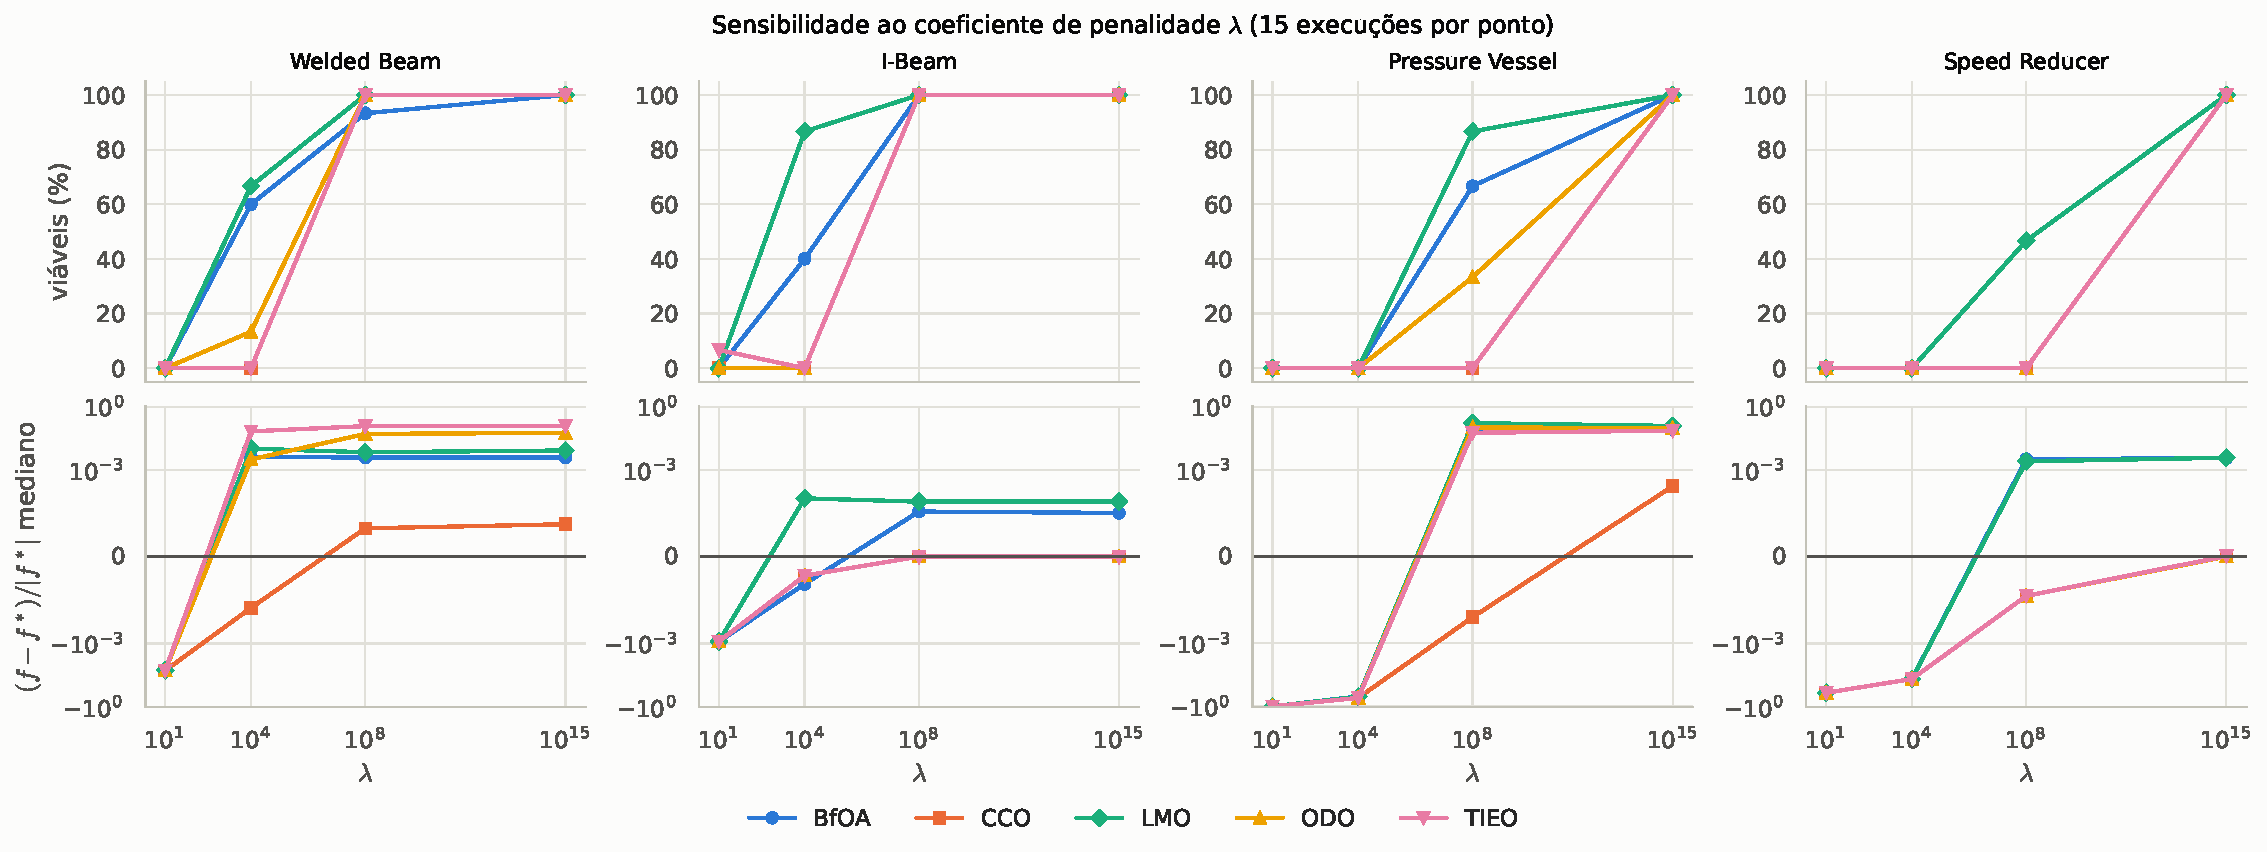
\includegraphics[width=\textwidth]{fig_exp_c_lambda}
  \caption{Exp.~C — sensibilidade ao coeficiente de penalidade $\lam$
           (15 execuções/ponto): taxa de viabilidade (\%, linha superior) e
           erro relativo mediano (linha inferior, escala \textit{symlog}).
           Todos os algoritmos atingem $100\%$ de viabilidade com $\lambda = 10^{15}$.}
  \label{fig:exp_c_lambda}
\end{figure}

% ═══════════════════════════════════════════════════════════════════════
\section{Experimento D — Escalabilidade}

\subsection{Contexto}

O Exp.~D avalia os algoritmos em seis funções deslocadas e rotacionadas
no estilo CEC~2017 (Bent~Cigar, Zakharov, Rosenbrock, Rastrigin, Levy,
Griewank), com dimensões $D \in \{10, 30, 50\}$ e orçamento
$\nfe_{\max} = 1000D$. Não há restrições e a rotação aleatória $\mathbf{M}$
destrói a separabilidade de todos os algoritmos.

\subsection{Resultados por função e dimensão}

A tabela~\ref{tab:exp_d} apresenta os valores medianos da função
objetivo (30 execuções) para cada configuração.

\begin{table}[h!]
\centering
\caption{Exp.~D — mediana do valor da função objetivo (sem restrições).
  Os menores valores por linha são em negrito.}
\label{tab:exp_d}
\small
\begin{tabular}{llrrrrr}
\toprule
$D$ & Função & \alg{BfOA} & \alg{CCO} & \alg{LMO} & \alg{ODO} & \alg{TIEO} \\
\midrule
\multirow{6}{*}{10}
 & Bent Cigar  & 3{,}48e+4 & \textbf{3{,}90e+3} & 2{,}16e+5 & 3{,}71e+3 & 6{,}77e+3 \\
 & Zakharov    & 1{,}40e-1 & \textbf{4{,}42e-2} & 4{,}30e+0 & 1{,}84e+3 & 3{,}33e+2 \\
 & Rosenbrock  & \textbf{4{,}50e+0} & 4{,}97e+0 & 7{,}41e+0 & 7{,}29e+0 & 5{,}66e+0 \\
 & Rastrigin   & 4{,}68e+1 & 1{,}25e+1 & \textbf{1{,}14e+1} & 2{,}29e+1 & 1{,}46e+1 \\
 & Levy        & 3{,}70e+0 & 8{,}95e-3 & 1{,}09e-2 & \textbf{5{,}65e-9} & 5{,}46e-2 \\
 & Griewank    & 4{,}25e-1 & \textbf{8{,}50e-2} & 6{,}24e-1 & 6{,}42e-1 & 4{,}92e-2 \\
\midrule
\multirow{6}{*}{30}
 & Bent Cigar  & 4{,}74e+5 & 7{,}37e+3 & 2{,}40e+6 & 7{,}60e+3 & \textbf{5{,}55e+3} \\
 & Zakharov    & \textbf{4{,}74e+1} & 1{,}22e+3 & 5{,}92e+3 & 5{,}88e+4 & 3{,}33e+4 \\
 & Rosenbrock  & 4{,}74e+1 & \textbf{2{,}63e+1} & 3{,}75e+1 & 3{,}64e+1 & 3{,}68e+1 \\
 & Rastrigin   & 1{,}65e+2 & 8{,}53e+1 & \textbf{5{,}40e+1} & 1{,}93e+2 & 5{,}58e+1 \\
 & Levy        & 6{,}46e+1 & 1{,}29e+1 & \textbf{3{,}58e-1} & 2{,}79e+0 & 1{,}32e+1 \\
 & Griewank    & 6{,}87e-1 & \textbf{9{,}51e-3} & 9{,}97e-1 & \textbf{8{,}37e-3} & 1{,}66e-2 \\
\midrule
\multirow{6}{*}{50}
 & Bent Cigar  & 2{,}74e+6 & \textbf{5{,}56e+3} & 7{,}67e+6 & 9{,}58e+5 & 6{,}83e+3 \\
 & Zakharov    & 8{,}42e+2 & \textbf{5{,}62e+3} & 5{,}01e+4 & 1{,}43e+5 & 9{,}71e+4 \\
 & Rosenbrock  & 1{,}61e+2 & \textbf{1{,}73e+2} & 1{,}67e+2 & 1{,}67e+2 & 1{,}86e+2 \\
 & Rastrigin   & 3{,}34e+2 & 1{,}92e+2 & \textbf{1{,}03e+2} & 3{,}98e+2 & 1{,}13e+2 \\
 & Levy        & 1{,}05e+2 & 4{,}64e+1 & \textbf{1{,}07e+0} & 7{,}83e+0 & 3{,}61e+1 \\
 & Griewank    & 8{,}67e-1 & \textbf{9{,}99e-3} & 1{,}06e+0 & 6{,}38e-1 & \textbf{1{,}42e-2} \\
\bottomrule
\end{tabular}
\end{table}

\subsection{Rankings por dimensão e teste de Friedman}

\begin{table}[h!]
\centering
\caption{Exp.~D — postos médios de Friedman por dimensão.}
\label{tab:rank_d}
\small
\begin{tabular}{lrrrrr}
\toprule
Dimensão & \alg{BfOA} & \alg{CCO} & \alg{LMO} & \alg{ODO} & \alg{TIEO} \\
\midrule
$D = 10$ ($N=6$)  & 3{,}33 & \textbf{1{,}83} & 3{,}50 & 3{,}33 & 3{,}00 \\
$D = 30$ ($N=6$)  & 3{,}83 & 2{,}17 & 3{,}17 & 3{,}00 & \textbf{2{,}83} \\
$D = 50$ ($N=6$)  & 3{,}17 & \textbf{2{,}50} & 3{,}00 & 3{,}33 & 3{,}00 \\
Todas ($N=18$)    & 3{,}44 & \textbf{2{,}17} & 3{,}22 & 3{,}22 & 2{,}94 \\
\bottomrule
\end{tabular}
\end{table}

Nenhuma das comparações do Exp.~D é estatisticamente significativa:
$D=10$: $\chi^2_F = 4{,}40$ ($p = 0{,}355$), $F_{ID} = 1{,}12$
($p = 0{,}374$);
$D=30$: $\chi^2_F = 3{,}47$ ($p = 0{,}483$), $F_{ID} = 0{,}84$
($p = 0{,}514$);
$D=50$: $\chi^2_F = 0{,}93$ ($p = 0{,}920$), $F_{ID} = 0{,}20$
($p = 0{,}934$);
Todas ($N=18$): $\chi^2_F = 7{,}16$ ($p = 0{,}128$), $F_{ID} = 1{,}88$
($p = 0{,}125$). Nenhum par é distinguível pelo teste de Nemenyi em
qualquer dimensão.

Embora o \alg{CCO} apresente os menores postos em $D=10$ e $D=50$
(e seja competitivo em $D=30$) e o \alg{BfOA} os maiores em $D=30$
e $D=50$, as diferenças entre algoritmos não são estatisticamente
significativas. O orçamento $\nfe_{\max} = 1000D$ (10\% do padrão CEC)
é claramente insuficiente para discriminar os algoritmos em funções
sem restrições — todos permanecem longe do ótimo, especialmente em
$D = 50$ com funções multimodais como Rastrigin e Levy.

\begin{figure}[H]
  \centering
  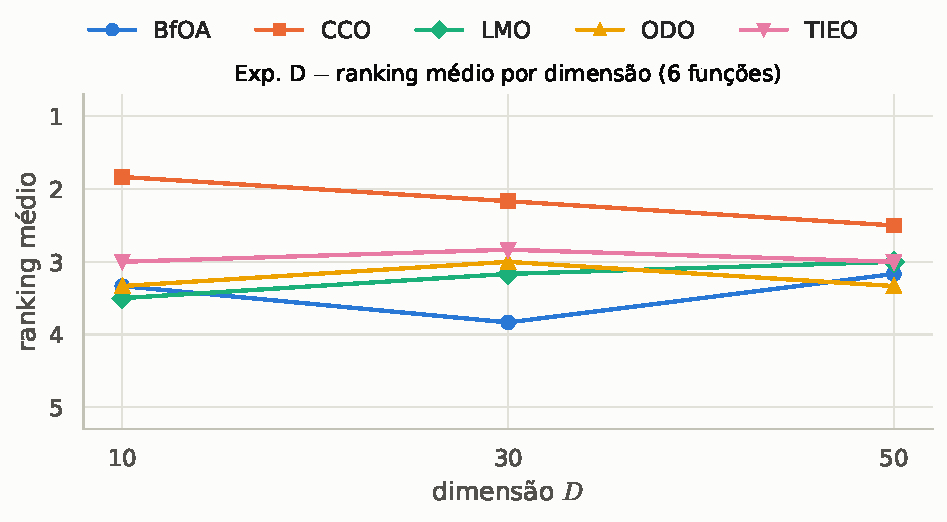
\includegraphics[width=0.62\textwidth]{fig_exp_d_ranking}
  \caption{Exp.~D — posto médio de Friedman por dimensão $D$ (menor = melhor).
           Nenhuma diferença é estatisticamente significativa ($p > 0{,}12$
           em todos os testes).}
  \label{fig:exp_d_ranking}
\end{figure}

% ═══════════════════════════════════════════════════════════════════════
\section{Conclusões Gerais}

\begin{enumerate}
  \item \textbf{O \alg{CCO} é o melhor algoritmo no contexto avaliado.}
    Obtém ranking~1 em todos os experimentos com restrições (Exps.~A,
    B e~C), com saldo $+28$ nas comparações por pares (WTL), e nunca
    perde para outro algoritmo nos Exps.~A e~B. Apresenta o menor
    desvio padrão (e.g., DP~$\approx 10^{-12}$ no Welded Beam),
    indicando busca extremamente consistente e precisa.

  \item \textbf{O protocolo original favorece o \alg{BfOA}} (ranking
    artigo: $4{,}2$) artificialmente, pois ele consome ${\approx}10\%$
    mais avaliações por iteração. Com orçamento equalizado no Exp.~B,
    o \alg{BfOA} permanece em 3º~lugar e o \alg{CCO} sobe para 1º.

  \item \textbf{Os valores reportados no artigo são inconsistentes
    com as reimplementações.} O \alg{LMO} apresenta média
    $\mu_{\text{artigo}} = 1{,}37\times10^{12}$ no Welded Beam
    (vs.\ $\mu_{\text{reprod.}} = 1{,}747$), e o I-Beam usa uma
    formulação com erro tipográfico ($f^{*\,\text{artigo}} = 0{,}0131$
    vs.\ $f^{*\,\text{correto}} = 0{,}01307$).

  \item \textbf{Penalidade $\lambda=10^{15}$ e regras de Deb produzem
    desempenho similar} no conjunto de problemas avaliado (tabela~WTL
    quase idêntica entre as duas estratégias). Ambas garantem $100\%$
    de viabilidade com $\nfe_{\max} = 15\,000$. A diferença
    metodologicamente relevante é que Deb garante viabilidade por
    construção, enquanto a penalidade requer $\lambda$ suficientemente
    grande — e $\lambda = 10^8$ é insuficiente para Pressure Vessel
    e Speed Reducer na maioria dos algoritmos.

  \item \textbf{Com $N=8$ problemas (Exp.~C), o teste de Friedman
    discrimina mais pares:} \alg{CCO} é separado de \alg{BfOA},
    \alg{LMO} e (com Deb) \alg{TIEO} pela diferença crítica
    ($\mathrm{CD} \approx 2{,}16$). Com apenas $N=5$ (Exps.~A e~B),
    apenas o par \alg{CCO}--\alg{LMO} é distinguível.

  \item \textbf{A escalabilidade em funções sem restrições (Exp.~D)
    não é discriminada com o orçamento disponível.} Nenhuma diferença
    entre algoritmos é estatisticamente significativa em qualquer
    dimensão ($p > 0{,}12$ em todos os testes). Rankings flutuam entre
    execuções e não há dominância estável, sugerindo que o orçamento
    $\nfe_{\max} = 1000D$ é insuficiente para separar os algoritmos
    nesse contexto.
\end{enumerate}

\end{document}
